
\begin{figure*}%[b]
\begin{center}
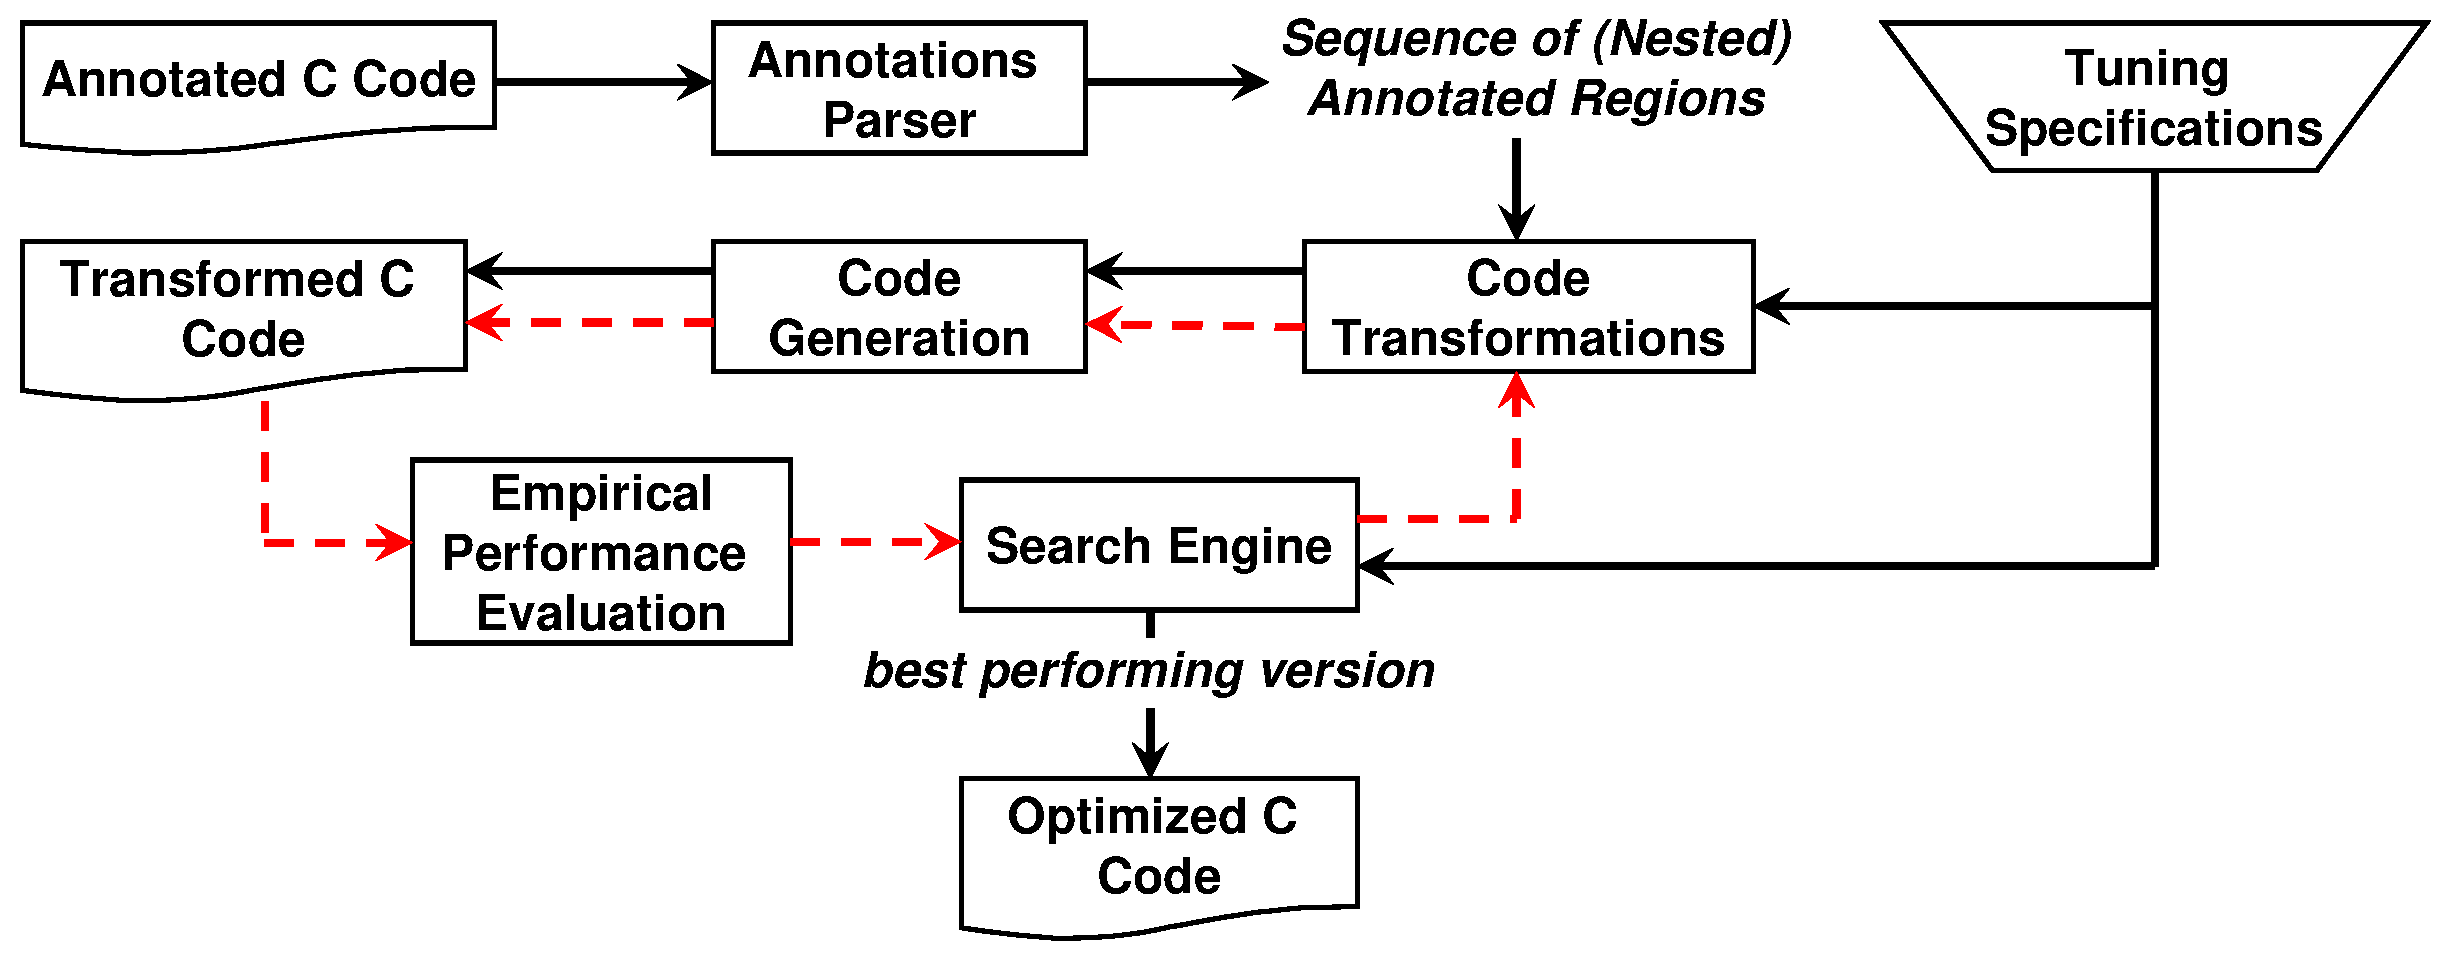
\includegraphics[width=0.6\textwidth]{figures/orio.eps}   
\end{center}
\caption{Overview of Orio's code generation and empirical tuning process.}  
\label{fig:orio}
\end{figure*}  

\begin{figure*}%[b]
\begin{center} 
\begin{tabular}{rrl} 
$<$annotation-region$>$ & ::= & $<$leader-annotation$>$ $<$annotation-body$>$ $<$trailer-annotation$>$\\ 
$<$leader-annotation$>$ & ::= & \texttt{/*@ begin} $<$module-name$>$ \texttt{(} $<$module-body$>$ \texttt{) @*/} \\
$<$trailer-annotation$>$ & ::= & \texttt{/*@ end @*/} \\
\end{tabular} 
\end{center}  
\caption{Annotation language grammar excerpt.}  
\label{fig:ann-lang}
\end{figure*}  

\section{Orio Design and Implementation}
\label{sec:implm}

Orio~\cite{OrioURL} is an empirical performance tuning system that takes
annotated C source code as input, generates many optimized code variants of
the annotated code, and empirically evaluates the performance of the
generated codes, ultimately selecting the best performing version to use for
production runs.

The Orio annotation approach differs from existing compiler- and
annotation-based systems in the following significant ways.
%
First, by not committing to a single general-purpose language, we can define 
annotation grammars that \emph{restrict} the original syntax, enabling more
effective performance transformations (e.g., disallowing pointer arithmetic
in a C-like annotation language); furthermore, it enables the definition of
new high-level languages which retain domain-specific
information that is normally lost in low-level C or Fortran
implementations. This in turn expands the range of possible performance-improving 
transformations.
%
Second, Orio was conceived and designed with the following requirements in mind: 
portability (which precludes extensive dependencies on external packages),
extensibility (new functionality must require little or no change to the
existing Orio implementation and interfaces that enable integration with
other source transformation tools must be defined), and automation
(ultimately Orio should provide tools that manage
\emph{all} the steps of the performance tuning process, automating each step 
as much as possible).
%
Finally, Orio is usable in real scientific applications without
requiring reimplementation. This ensures that the significant investments in
the development of complex scientific codes is leveraged to the greatest
extent possible.

Figure~\ref{fig:orio} contains a high-level graphical depiction of the code
generation and tuning process implemented in Orio.  Orio can be used to
improve performance by source-to-source transformations such as loop
unrolling, loop tiling, and loop permutation. The input to Orio is C code
containing structured comments that include a simplified expression of the
computation, as well as various performance-tuning directives. Orio scans the
marked-up input code and extracts all annotation regions. Each annotation
region is then processed by transformation modules. The code generator then
produces the final C code with various optimizations that correspond to the
specified annotations. Unlike compiler approaches, we do not implement a
full-blown C compiler; rather, we use a precompiler that parses only the
language-independent annotations.

Orio can also be used as an automatic performance tuning tool.  The code
transformation modules and code generator produce an optimized code version
for each distinct combination of performance parameter values. Then each
optimized code version is executed and its performance evaluated.  After
iteratively evaluating all code variants, the best-performing code is picked
as the final output of Orio. Because the search space of all possible
optimized code versions can be huge, a brute force search strategy is not
always feasible. Hence, Orio provides various search heuristics for reducing
the size of the search space and thus the empirical testing time.

%% BN: The info in the paragraph below is repeated later in the discussion.
%The tuning specifications written by users in the form of annotations
%are parsed and used by Orio to guide the transformations and the
%empirical tuning process. These specifications include essential
%information such as the used base compilers, the search strategy, the
%program transformation parameters, the input data sizes, etc.

\subsection{Annotation Language Syntax} 
\label{sec:ann-lang}

Orio annotations are embedded into the source code as structured C comments
that always start with \texttt{/*@} and end with \texttt{@*/}. For example,
the annotation \texttt{/*@ end @*/} is used to indicate the end of an
annotated code region. A simple grammar illustrating the basic syntax of Orio
annotations is depicted in Figure~\ref{fig:ann-lang}. An annotation region
consists of three main parts: leader annotation, annotation body, and trailer
annotation. The annotation body can be either empty or contain C code that
possibly includes other nested annotation regions. A leader annotation
contains the name of the code transformation module used to transform and
generate the annotated application code. A high-level description of the
computation and several performance hints are coded in the module body inside
the leader annotation. A trailer annotation, which has a fixed form (i.e.,
\texttt{/*@ end @*/}), closes an annotation region.

\subsection{Orio Input Example}
\label{sec:example}

Figure~\ref{fig:orio-example} shows a concrete annotation example that
empirically optimizes a C function for the Blue Gene/P
architecture. This is an instance of an AXPY operation, i.e., one that computes
$y=y+a_1 x_1+\cdots+a_n x_n$, where $a_1,\ldots,a_n$ are scalars and
$y,x_1,\ldots,x_n$ are one-dimensional arrays. The specific AXPY operation
considered in this example corresponds to $n=4$. The first annotation contains the
\texttt{BGP\_Align}\footnote{Architecture-specific annotations are simply ignored when the
code is being tuned on an architecture that doesn't support them.} directive,
which instructs Orio to dynamically load its memory-alignment optimization
module and then generate preprocessor directives, such as pragmas and calls
to memory alignment intrinsics, including a check for data alignment. The
main purpose of these alignment optimizations is to enable the use of the
dual floating-point unit (Double Hummer) of the Blue Gene/P, which requires
16-byte alignment. As discussed later in Section~\ref{sec:axpy4-results},
even these simple alignment optimizations can lead to potentially significant
performance improvements. This example also shows the use of Orio's loop
transformation module (named \texttt{Loop}) to optimize the AXPY-4 loop by
unrolling and generating OpenMP parallelization directives for exploiting
multicore parallelism. In addition to the simple source transformations in
this example, Orio also supports other optimizations, such as register
tiling and scalar replacement.

Whereas the \texttt{BGP\_Align} and \texttt{Loop} annotations in this example
guide the source-to-source transformations, the purpose of the
\texttt{PerfTuning} annotation is primarily to control the empirical
performance tuning process. Details of the tuning specifications for
optimizing the AXPY-4 code on Blue Gene/P are shown in the right-hand side of
Figure~\ref{fig:orio-example}.  The tuning specification contains data
required for building, initializing, and running experiments, including input
variable information, the search algorithm, performance counting technique,
performance parameters values, and execution environment details.  The tuning
specifications can be either integrated in the source code or defined in a
separate file, as in this example.

\begin{figure*}%[!t] 
\centering 
\begin{tabular}{cc} 
\begin{minipage}{.5\textwidth}  
\scriptsize
\begin{verbatim}  
 void axpy4(int N, double *y, 
  double a1, double *x1, double a2, double *x2, 
  double a3, double *x3, double a4, double *x4) {

  /*@ begin PerfTuning (
    import spec axpy4_tune_spec;
  ) @*/

  register int i;

  /*@ begin BGP_Align (x1[],x2[],x3[],x4[],y[]) @*/ 
  /*@ begin Loop ( 
   transform Unroll (ufactor=UF, parallelize=PAR)
   for (i=0; i<=N-1; i++) 
     y[i] += a1*x1[i]+a2*x2[i]+a3*x3[i]+a4*x4[i]; 
  ) @*/ 

  for (i=0; i<=N-1; i++) 
    y[i] += a1*x1[i]+a2*x2[i]+a3*x3[i]+a4*x4[i];

  /*@ end @*/ 
  /*@ end @*/
  /*@ end @*/
 }









\end{verbatim}  
\end{minipage}
&
\begin{minipage}{.5\textwidth}  
\scriptsize
\begin{verbatim}  
 spec axpy4_tune_spec {
  def build { 
   arg build_command = 
    'mpixlc_r -O3 -qstrict -qhot -qsmp=omp:noauto'; 
   arg batch_command = 
    'qsub -n 128 -t 20 --env "OMP_NUM_THREADS=4"'; 
   arg status_command = 'qstat';
   arg num_procs = 128; 
  } 
  def performance_counter { 
   arg method = 'basic timer';
   arg repetitions = 10000;
  } 
  def performance_params { 
   param UF[] = range(1,33);
   param PAR[] = [True,False]; 
  }
  def input_params { 
   param N[] = [10,100,1000,10**4,10**5,
                10**6,10**7]; 
  }
  def input_vars { 
   decl dynamic double y[N] = 0; 
   decl dynamic double x1[N] = random; 
   decl double a1 = random; 
   decl double a2 = random; 
   # ... ommitted ...
  } 
  def search { 
   arg algorithm = 'Exhaustive'; 
   arg time_limit = 20;
  }
 }
\end{verbatim}  
\end{minipage}
\\
\end{tabular}
\caption{Orio input example; annotated AXPY-4 source code (left) and tuning specification for the Blue Gene/P (right).}
\label{fig:orio-example}  
\end{figure*} 

\begin{figure*}%[!t] 
\centering 
\begin{tabular}{cc} 
\begin{minipage}{.5\textwidth}  
\scriptsize
\begin{verbatim}  
 /*@ begin Loop (
 transform UnrollJam(ufactor=Ui)
 for (i=0; i<=M-1; i++)
   transform UnrollJam(ufactor=Uj)
   for (j=0; j<=N-1; j++)
     transform UnrollJam(ufactor=Uk)   
     for (k=0; k<=O-1; k++)
       A[i][j] += B[i][k]*C[k][j];
 ) @*/
 for (i=0; i<=M-1; i++)
  for (j=0; j<=N-1; j++)
   for (k=0; k<=O-1; k++)
     A[i][j] += B[i][k]*C[k][j];
 /*@ end @*/
\end{verbatim}  
\end{minipage}
&
\begin{minipage}{.5\textwidth}  
\scriptsize
\begin{verbatim}  
 def performance_params {
   param Ui[] = range(1,33);
   param Uj[] = range(1,33);
   param Uk[] = range(1,33);
   constraint reg_capacity = Ui*Uj+Ui*Uk+Uk*Uj<=32;
 }

 def input_params {
   param M[] = [10,50,100,500,1000];
   param N[] = [10,50,100,500,1000];
   param O[] = [10,50,100,500,1000];
   constraint square_matrices = (M==N) and (N==O);
 }

\end{verbatim}  
\end{minipage}
\\
\end{tabular}
\caption{Example of specifying parameter constraints in Orio; annotated code for matrix-matrix multiplication (left) and constraint specification (right).}
\label{fig:par-constraint}  
\end{figure*} 

The annotated AXPY-4 code (left side of Figure~\ref{fig:orio-example}) uses two
performance parameters whose values are defined in the tuning specification:
the unroll factor (\texttt{UF})
% which signifies how many times the loop body will be
%replicated in the generated code.
and the boolean variable \texttt{PAR}, which is used to activate or
deactivate OpenMP parallelization. 
%Such boolean parameter is needed by Orio
%due to the following basis: when both the number of loop iterations and the
%total amount of computation in the loop body are small, parallelizing a loop
%using OpenMP can give poor performance because of the dominating overhead
%incurred from thread coordination and task scheduling. Therefore, based on a
%given vector size, Orio can determine at runtime whether it is beneficial to
%parallelize the loop.
These parameters are used by Orio to determine at runtime whether it is
beneficial to parallelize the loop, i.e., whether there is enough work per
thread to offset the OpenMP overhead or not.

Achieving the best performance for different input problem sizes may require
different tuning approaches; thus, the entire tuning process is
repeated for each specified problem size. In the AXPY-4 example, the search
space includes seven different input problem sizes (variable~\texttt{N}). 
%Orio repeats the tuning process for each problem size, resulting
%in the generation of seven final optimized codes.

\subsection{Annotation Parsing and Code Generation}

The Orio system consists of several optimization modules, each implemented as
a Python module. As mentioned earlier in Section~\ref{sec:example}, given the
module name in the leader annotation, Orio dynamically loads the
corresponding code transformation module and uses it for both annotation
parsing and code generation. If the pertinent module cannot be found in the
transformation modules directory, an error message is emitted and the tuning
process is terminated. This name-based dynamic loading provides flexibility
and easy extensibility without requiring detailed knowledge or modification
of the existing Orio software. Therefore, varied approaches to code
transformations ranging from low-level loop optimizations for cache
performance to composed linear algebra operations and new specialized
algorithms can easily be integrated into Orio.

%Taking as input the information supplied in both the annotation body
%and the module body, 
After parsing the annotation, each module performs a distinct optimization
transformation prior to generating the optimized code.  The transformation
module can either reuse an existing annotation parser or define new language
syntax and a corresponding parser component. 

%%BN: the details below are probably not essential for this paper
%In some cases, the annotation is seemingly redundant, containing a version of
%the computation that is very similar to the original code. 
%We took this
%approach for two reasons.  First, basing the transformation modules on the
%actual application code demands a full-fledged C compiler
%infrastructure. Requiring this complex compiler infrastructure to avoid a
%relatively small manual effort in creating annotations runs counter to our
%goal of creating the annotation system portable and easy to install and
%use. Second, requiring in effect a rewrite of the code to be optimized
%encourages simplification and enables the code optimization effort to start
%with a cleaner, rather than an already hand-tuned, version of the
%code. Moreover, we are investigating higher-level, domain-specific syntax for
%annotations, thus capturing semantics without imposing tuning constraints
%resulting from the use of the general-purpose C language. 
In some cases, the annotation is seemingly redundant, containing a version of
the computation that is very similar to the original code.  As mentioned
earlier, we took this approach so that the annotation language can be defined
in a way that enables more effective transformations (through restrictions or
high-level domain information).

Current optimizations supported by Orio span different types of code
transformations that are not provided by production compilers in some
cases. Available optimizations include simple loop unrolling, memory
alignment optimization, loop unroll/jamming, loop tiling, loop permutation,
scalar replacement, register tiling, loop-bound replacement, array copy
optimization, multicore parallelization (using OpenMP), and other
architecture-specific optimizations (e.g., generating calls to SIMD
intrinsics on Intel and Blue Gene/P architectures).

\subsection{Search Space Exploration and Evaluation}
\label{sec:search-space}

As briefly discussed earlier, our empirical tuning approach systematically
measures the performance costs of automatically-generated code variants in
order to find the most optimal available version. In the context of empirical
optimization, code variants are alternative, semantically equivalent
implementations of the same computation. Each implementation variant is
associated with a collection of different optimization parameters that
correspond to source-to-source code transformations such as, for instance,
unroll factors, tile sizes, and loop permutation order. So, each coordinate
in the search space of empirical tuning problem represents a distinct
combination of performance parameter values. Both the dimension and the size
of the search space depend on the total number and the value ranges of used
performance parameters, respectively.

The conceptually straightforward approach to exploring the space of the
parameter values is to use an exhaustive search procedure that is guaranteed
to find the optimal code version. Normally the size of the search space
is too large, making full coverage impractical.  Thus, in addition to
supporting exhaustive search, we have implemented several search heuristics.
The simplest search heuristic is a random search, which picks a random
coordinate in the search space at each step and then measures its
performance; random search is not guaranteed to return close-to-optimal results.
We have also developed two other search heuristics to effectively
narrow the search space for close-to-optimal performance, including a
heuristic based on the \textit{Nelder-Mead simplex}
method~\cite{Lagarias98simplex,Lewis00directsearch}, 
a popular non-derivative direct search method for optimization, and \textit{simulated
annealing}\cite{Kirkpatrick83optimizationby}.
%with the additional inclusion of
%a gradually-reduced ``temperature'' used to control the randomness of
%selecting the next move in the search space. 
%By default Orio uses exhaustive
%search, but users can set the search parameters in the tuning specification
%to use and configure one of the available heuristics.  
Similarly to the implementation of Orio's optimization modules, each search
technique is implemented as an independent Python module in Orio and is dynamically
loaded given only the algorithm's name as one of the fields in the tuning
specification.

%%BN: commenting for space
%The key idea of a basic simplex method
%is to construct a nondegenerate simplex (i.e., a convex hull of $n+1$ points,
%where $n$ is the dimension of the search space), and then obtain its
%associated function values to steer the search to the next move by replacing
%the worst vertex with a point reflected through the centroid of the remaining
%$n$ points. The simplex search is improved in the Nelder-Mead method by
%adding more moves, making the search more robust and faster to converge. \

%The exhaustive approach is chosen as the default space exploration
%method of Orio; however, users can switch to the other algorithms by
%manually indicating his preferred search strategy in the tuning
%specifications. Users can also specify terminating criteria of the
%chosen search strategy by providing numerical values to the search
%time limit and the maximum total number of search trials. Each time
%the search exceeds the specified time limit or the predetermined
%number of full search runs, we suspend the search and return the best
%implementation variant up to that point of time. Also, users can
%optionally adjust the search by altering the values of some
%algorithm-specific parameters in the tuning specifications. As an
%example, users can change four types of coefficients that the
%Nelder-Mead simplex method has: reflection, expansion, contraction,
%and shrinkage, in order to control the search convergence speed and
%the quality of the search outcome.

To improve the quality of the search result further, each search heuristic is
enhanced by applying a local search after the global search completes. The
local search compares the best performance with neighboring coordinates. If a
better coordinate is discovered, the local search continues recursively until
no further performance improvement is possible or a user-specified
termination criterion is met.

Further pruning of the search space is enabled through user-specified
constraints in the tuning specifications. We use loop the
unroll/jamming transformation to make the discussion more concrete. Loop
unroll/jamming~\cite{sarkar-unrolljam} (coupled with scalar replacement) is
mainly intended to increase data reuse at the register level. So, when
unroll/jamming is applied to multiple loops, the values of unroll factors
must be such that register locality is maximized while satisfying the
register capacity constraints to avoid unnecessary register
spills. Figure~\ref{fig:par-constraint} shows an example of analytically
enforcing register capacity constraints on matrix-matrix multiplication code
that is optimized with loop unroll/jamming, assuming 32
registers. \texttt{Ui}, \texttt{Uj}, \texttt{Uk} are unroll factors for loops
\texttt{i}, \texttt{j}, \texttt{k}, respectively. With the specified
parameter constraints, the search space of performance parameter values is
drastically trimmed down from 32,768 points (i.e., $32*32*32$) to only 65
points. This example also demonstrates that a set of constraints can also be
imposed on input parameters to decide what input problem sizes to consider.

Orio also supports parallel search when parallel resources are
available, e.g., when tuning on the Blue Gene/P. The parallel Orio
driver concurrently executes multiple independent code variants in the
same parallel job. After Orio submits a parallel job, each node in the
target machine executes a distinct generated code variant to collect
the code performance. The resulting performance results are collected
and stored in a temporary file, which is later processed by Orio to
determine the best performing variant.  Figure~\ref{fig:orio-example}
has an example of using parallel search by specifying the number of
nodes to use (per job) with the \texttt{num\_procs} variable. The
remaining fields used by the parallel search are the
\texttt{batch\_command} and the \texttt{status\_command} fields, which
specify how Orio should submit a parallel job and query its status,
respectively.

